%%%%%%%%%%%%%%%%%%%% author.tex %%%%%%%%%%%%%%%%%%%%%%%%%%%%%%%%%%%
%
% sample root file for your "contribution" to a proceedings volume
%
% Use this file as a template for your own input.
%
%%%%%%%%%%%%%%%% IEEE %%%%%%%%%%%%%%%%%%%%%%%%%%%%%%%%%%


\documentclass[conference]{IEEEtran}

% Force numeric author reference marks (1,2,3,...) instead of symbol marks (*,†,‡,...)
\makeatletter
\renewcommand{\IEEEauthorrefmark}[1]{\textsuperscript{#1}}
\makeatother
%
% RECOMMENDED %%%%%%%%%%%%%%%%%%%%%%%%%%%%%%%%%%%%%%%%%%%%%%%%%%%
%

% to typeset URLs, URIs, and DOIs
\usepackage{url}
\usepackage{color}
\usepackage{graphicx}        % standard LaTeX graphics tool
\usepackage{tabularx}
\usepackage{multirow}
\usepackage{cite}
\usepackage{algorithm}
\usepackage{algorithmic}
\usepackage{longtable}
\usepackage{rotating}
\usepackage{placeins}
 \usepackage{amsmath}
\usepackage{amssymb}
\def\UrlFont{\rmfamily}

\begin{document}
%
\title{ML-Based Decision Support System\\for Smart Investments}
\author{\IEEEauthorblockN{Dr. Reshma Koli\IEEEauthorrefmark{1}, Avanish Vadke\IEEEauthorrefmark{2}, Atharva Shelke\IEEEauthorrefmark{3},\\Abhishek Thormothe\IEEEauthorrefmark{4}, Aadit Suryawanshi\IEEEauthorrefmark{5},\\Prof. Harshada Sonkamble\IEEEauthorrefmark{6}}
\IEEEauthorblockA{\IEEEauthorrefmark{1}\IEEEauthorrefmark{2}\IEEEauthorrefmark{3}\IEEEauthorrefmark{4}\IEEEauthorrefmark{5}\IEEEauthorrefmark{6}A.P. Shah Institute of Technology, Thane, India\\
rrkoli@apsit.edu.in, avanishvadke3@apsit.edu.in,\\
atharvashelke2@apsit.edu.in, abhishekthormothe150@apsit.edu.in,\\
aaditsuryavanshi60@apsit.edu.in, hksonkamble@apsit.edu.in}}

\maketitle              % typeset the title of the contribution

\begin{abstract}
Retail investors and discretionary traders make decisions under uncertainty, limited information, and behavioral bias; without a measurable workflow, these decisions can lead to avoidable drawdowns. This paper presents \emph{QuantFin}, a machine learning--based decision support system for equity investments targeting Indian large-cap stocks (Nifty~50 constituents available in our dataset). QuantFin integrates: (i) reproducible ingestion of OHLCV time series from multi-header CSV exports; (ii) a technical-indicator feature pipeline; (iii) a multi-model prediction stack (ridge regression, logistic regression, support vector machines (SVM), ARIMA, and long short-term memory (LSTM)) used for forecasting and comparison; (iv) portfolio construction via ML-driven ranking and optimization-based baselines; and (v) walk-forward backtesting that evaluates rebalanced strategies against a benchmark under leakage-aware date cutoffs.

The system is implemented as a FastAPI backend exposing portfolio, analytics, prediction, and backtest endpoints, coupled with a React/TypeScript dashboard. We report results produced by the repository's own training logs and backtest engine. For example, on the RELIANCE dataset, saved training metrics show test accuracy of 0.5003 (logistic regression) and 0.5136 (SVM) for directional classification, and LSTM test MAPE of 20.447\% for price forecasting. In a reproducible walk-forward run (monthly rebalancing, 2023-01-01 to 2024-01-01), the implemented LINEAR strategy achieved CAGR 48.31\% versus 30.60\% for the benchmark under the repository's assumptions.
\end{abstract}

\begin{IEEEkeywords}
Decision Support Systems, Quantitative Finance, Portfolio Construction, Walk-Forward Backtesting, Time Series Forecasting, FastAPI, Nifty~50
\end{IEEEkeywords}
%
\section{Introduction}\label{sec:intro}
Quantitative investing systems increasingly combine statistical modeling, machine learning, and portfolio construction under realistic evaluation. Recent IEEE and Springer literature covers both end-to-end portfolio decision support systems and algorithmic techniques for portfolio construction and ranking \cite{aithal2023realtime,gunjan2022portfolioreview,saha2021stockranking}. A recurring theme is that reported performance is sensitive to evaluation protocol: time-order must be respected and realistic constraints (e.g., rebalancing cadence and capital limits) must be explicit.

QuantFin is designed as a full-stack platform that connects these components for the Indian equity universe (Nifty~50 constituents available in the repository dataset). Unlike isolated notebooks, QuantFin operationalizes a repeatable workflow: (i) ingestion of OHLCV data from CSV exports with robust header handling; (ii) technical indicator generation; (iii) model training and prediction orchestration across multiple approaches (ridge regression, logistic regression, SVM, ARIMA, LSTM); (iv) portfolio construction and rebalancing; and (v) walk-forward backtesting with a benchmark.

\textbf{Contributions.} The main contributions of this work are:
\begin{itemize}
\item An end-to-end, modular architecture (FastAPI backend + React/Vite dashboard) for interactive quantitative analysis.
\item A walk-forward backtesting procedure that enforces date cutoffs at each rebalance date (mitigating look-ahead bias) and reports risk-adjusted metrics.
\item A multi-model prediction layer and multiple portfolio construction baselines (ML-driven ranking, model-weighted allocation, mean--variance, risk parity) implemented in the repository.
\end{itemize}

\textbf{Paper organization.} Section~\ref{sec:system} describes system architecture; Section~\ref{sec:data} covers data and features; Section~\ref{sec:models} presents the model suite; Sections~\ref{sec:portfolio}--\ref{sec:backtest} describe portfolio construction and backtesting; Section~\ref{sec:exp} reports experiments; Section~\ref{sec:con} concludes.

\section{System Overview}\label{sec:system}
QuantFin is implemented as a modular full-stack system:
\begin{itemize}
\item \textbf{Backend:} a FastAPI service exposing endpoints for portfolio rebalancing, analytics (training + metrics), predictions, and walk-forward backtesting.
\item \textbf{Model services:} reusable components for data preprocessing, feature engineering, model training, prediction orchestration, and portfolio allocation.
\item \textbf{Frontend:} a React + TypeScript dashboard built with Vite that calls backend APIs and visualizes model performance, allocations, and time-series charts.
\end{itemize}

Figure~\ref{fig:arch} provides a conceptual architecture diagram.

\begin{figure}[h!]
\begin{center}
\fbox{\parbox{0.95\columnwidth}{
\textbf{QuantFin Architecture (conceptual).}\\
\emph{Data layer:} CSV OHLCV $\rightarrow$ preprocessing $\rightarrow$ feature engineering.\\
\emph{Model layer:} Linear, Logistic, SVM, ARIMA, and LSTM models with an ensemble option.\\
\emph{Decision layer:} portfolio weighting + rebalancing + backtesting.\\
\emph{Serving layer:} FastAPI endpoints consumed by a React dashboard.
}}
\caption{QuantFin system architecture.}
\label{fig:arch}
\end{center}
\end{figure}

\section{API and Service Design}\label{sec:api}
QuantFin exposes modular API surfaces aligned to internal services.
\begin{itemize}
\item \textbf{Portfolio endpoints} (prefix \url{/api/portfolio}): summary and performance series, portfolio health, rebalancing workflows, and cached strategy comparisons.
\item \textbf{Analytics endpoints} (prefix \url{/api/analytics}): background model training triggers (with status reporting), retrieval of cached model metrics, and candlestick/price-series endpoints backed by local OHLCV.
\item \textbf{Prediction endpoints} (prefix \url{/api/predictions}): per-symbol inference and portfolio recommendations parameterized by model family and prediction horizon.
\item \textbf{Backtest endpoints} (prefix \url{/api/backtest}): walk-forward evaluation via POST \url{/run}, returning portfolio and benchmark value series plus risk/return metrics.
\end{itemize}
The API layer is intentionally thin; request/response validation is performed via typed request/response models.

\section{Data and Feature Engineering}\label{sec:data}
QuantFin operates on daily OHLCV time series for Nifty~50 constituents stored as CSV files (one file per symbol). In the current repository state, the backend data directory contains 49 stock CSV files (excluding auxiliary files such as \texttt{nifty50.csv} and \texttt{tcs\_combined\_news.csv}). While a news CSV exists, it is explicitly excluded from the backend's stock-data loader and is not used by the current prediction or allocation flow.

\subsection{Preprocessing}
Market CSV files can contain multi-row headers depending on the export source. QuantFin includes preprocessing routines that normalize these files into a canonical schema with columns (Date, Open, High, Low, Close, Volume) and a datetime index. For example, the real-data service reads each symbol CSV with header skipping (\texttt{skiprows=3}), coerces numeric columns, drops invalid rows, sorts by date, and caches the result to reduce repeated I/O.

\subsection{Feature set}
The feature pipeline generates both return-based and indicator-based features commonly used in technical analysis:
simple and exponential moving averages (SMA/EMA), MACD, RSI, Bollinger bands, rolling volatility, lagged returns, momentum features, and volume features. In addition, log-returns are computed for stability in statistical modeling and walk-forward evaluation pipelines.

Given close price $P_t$, QuantFin uses simple returns and log-returns:
\begin{equation}
r_t = \frac{P_t - P_{t-1}}{P_{t-1}},\quad \ell_t = \log\left(\frac{P_t}{P_{t-1}}\right)
\end{equation}
These features are combined with indicators to form the model input matrix.

\section{Model Suite and Prediction Orchestration}\label{sec:models}
QuantFin supports complementary model families to address both regression and classification tasks.

\subsection{Ridge regression (linear)}
For regression targets, QuantFin trains a linear model with $\ell_2$ regularization (ridge regression). Given features $X \in \mathbb{R}^{n\times d}$ and targets $y \in \mathbb{R}^n$, ridge solves:
\begin{equation}
\hat{\beta} = \arg\min_{\beta} \|y - X\beta\|_2^2 + \alpha\|\beta\|_2^2
\end{equation}
where $\alpha > 0$ controls shrinkage. This choice is computationally efficient and mitigates multicollinearity among correlated indicators.
where $\alpha > 0$ controls shrinkage. This choice is computationally efficient and mitigates multicollinearity among correlated indicators.

\subsection{Logistic regression (directional classification)}
For directional classification (up/down), QuantFin trains logistic regression. With feature vector $x$ and label $y\in\{0,1\}$, the model estimates:
\begin{equation}
\Pr(y=1\mid x)=\sigma(w^\top x+b),\quad \sigma(z)=\frac{1}{1+e^{-z}}
\end{equation}
and optimizes regularized cross-entropy. This provides an interpretable classification baseline.

\subsection{Support vector machines}
Support vector machines (SVMs) provide a non-linear classification baseline via kernel methods. QuantFin includes an RBF-kernel SVM pipeline trained on engineered technical features. In the saved RELIANCE training log, the best hyperparameters were $C=10.0$ and $\gamma=0.01$.

\subsection{ARIMA}
ARIMA family models provide a classical statistical baseline for univariate time series. QuantFin includes an ARIMA training routine as a comparative baseline, consistent with recent studies that benchmark ARIMA alongside neural approaches \cite{gao2021arimadeep}.

\subsection{LSTM}
LSTM sequence models capture non-linear temporal patterns and can ingest windows of engineered features. QuantFin provides an LSTM implementation including sequence windowing, scaling, and early stopping. Recent IEEE work has applied LSTM-based architectures to stock trend prediction under time-ordered market data \cite{karlis2021lstmfusion}. For a sequence $(x_{t-L+1},\dots,x_t)$, an LSTM cell computes gated updates:
\begin{align}
f_t &= \sigma(W_f[x_t,h_{t-1}] + b_f),\quad i_t = \sigma(W_i[x_t,h_{t-1}] + b_i),\\
\tilde{c}_t &= \tanh(W_c[x_t,h_{t-1}] + b_c),\quad c_t = f_t\odot c_{t-1} + i_t\odot \tilde{c}_t,\\
o_t &= \sigma(W_o[x_t,h_{t-1}] + b_o),\quad h_t = o_t\odot \tanh(c_t)
\end{align}
where $f_t,i_t,o_t$ are forget/input/output gates and $c_t$ is the cell state.

\subsection{Prediction service}
A central prediction service loads trained models, generates per-symbol forecasts for a chosen horizon, and aggregates predictions for downstream allocation. The API supports both single-model inference and an ``ensemble'' option that aggregates signals across available model families. Ranking-based modeling and selection are commonly used in stock recommendation pipelines \cite{saha2021stockranking}.

\section{Portfolio Construction and Rebalancing}\label{sec:portfolio}
QuantFin exposes portfolio construction via both ML-driven ranking and optimization-based weighting.

\subsection{Model-driven ranking}
The repository implements ML-driven ranking in the portfolio allocator used by the \url{/api/portfolio/rebalance} endpoint. For each symbol, the allocator estimates a predicted return (in percent) and a confidence score derived from data characteristics (volatility regime, trend consistency, and data completeness). It ranks symbols by:
\begin{equation}
\mathrm{score}_i = \widehat{r}_i \cdot c_i
\end{equation}
filters out negative predicted returns, selects the top-$N$ symbols, and converts weights into integer share quantities under a capital budget.

\subsection{Mean--variance optimization}
For users who prefer optimization-based weighting, QuantFin supports mean--variance and risk-parity style allocations as baselines. In the current repository state, the 
prediction service's optimization routines use a simplified covariance structure (per-asset volatility estimates with a fixed pairwise correlation assumption), while the walk-forward backtest engine can estimate a covariance matrix empirically from historical returns over a rolling lookback window. Mean--variance style formulations remain a widely used baseline family in portfolio optimization research \cite{gunjan2022portfolioreview}.

\subsection{Rebalance procedure}
Rebalancing produces a set of target weights and quantities for a specified capital allocation. The backend persists portfolio metadata and exposes endpoints for summary and performance.

\begin{algorithm}
\caption{Leakage-aware monthly rebalancing (simplified)}
\label{alg:rebalance}
\begin{algorithmic}
\STATE Input: symbols $S$, rebalance dates $D$, horizon $h$, top-$N$.
\STATE Initialize capital $C_0$.
\FOR{$t = 1$ to $|D|-1$}
\STATE Cutoff date $d \leftarrow D[t]$.
\STATE For each $s \in S$: compute features using data $\le d$ and predict return $\hat{r}_{s}$.
\STATE Compute confidence $c_s$ from data quality/volatility/trend fit.
\STATE Rank by score $\hat{r}_{s}\cdot c_s$ and select top-$N$ with $\hat{r}_{s} > 0$.
\STATE Compute target weights and integer share quantities under capital $C_{t-1}$.
\STATE Realize return over $(D[t], D[t+1]]$ and update capital.
\ENDFOR
\STATE Output: portfolio value series and returns.
\end{algorithmic}
\end{algorithm}

\section{Walk-Forward Backtesting}\label{sec:backtest}
Backtesting is implemented as a walk-forward simulation: at each rebalance date, the system generates predictions using only historical data up to that date, constructs a portfolio, and then evaluates realized returns over the next period. This avoids look-ahead bias by construction.

QuantFin reports standard risk-adjusted metrics such as CAGR, Sharpe ratio, Sortino ratio, maximum drawdown, annualized volatility, Calmar ratio, and win rate. A benchmark portfolio is computed using an equal-weight basket over the available universe for the same rebalance periods. Periodic rebalancing and performance evaluation are standard in recent ML-based portfolio management studies \cite{lim2022dynamicrebalancing,aithal2023realtime}.

Given a portfolio value series $V_t$ and periodic returns $r_t=\frac{V_t-V_{t-1}}{V_{t-1}}$, the implemented evaluation reports:
\begin{equation}
\mathrm{CAGR} = \left(\frac{V_T}{V_0}\right)^{\tfrac{1}{Y}}-1,\quad \sigma = \sqrt{\mathrm{Var}(r_t)}\cdot\sqrt{K}
\end{equation}
where $Y$ is the number of years in the backtest and $K$ is the annualization factor for the return frequency. Sharpe and Sortino use excess returns over a risk-free rate $r_f$:
\begin{equation}
\mathrm{Sharpe} = \frac{\mathbb{E}[r_t-r_f/K]}{\sigma},\quad
\mathrm{Sortino} = \frac{\mathbb{E}[r_t-r_f/K]}{\sigma_-}
\end{equation}
where $\sigma_-$ is downside deviation computed over $\min(r_t,0)$.

\section{Experimental Results}\label{sec:exp}
This section summarizes representative training results generated by the QuantFin training pipeline.

\subsection{Training configuration}
Models are trained on engineered technical features and evaluated on held-out data. For time-series workflows, a time-based split is preferred to avoid leakage through shuffling.

\subsection{Reproducible artifacts (repo-grounded)}
QuantFin persists intermediate artifacts that make experimentation reproducible within the repository: (i) cached training summaries and per-symbol metrics in JSON files (e.g., \texttt{backend/training\_results.json}, \texttt{backend/training\_summary.json}); (ii) validation outputs (\texttt{backend/validation\_report.json}); and (iii) saved model weights for some families (e.g., pre-trained LSTM \texttt{.h5} files under \texttt{backend/models}).

\subsection{Sample model metrics}
Table~\ref{tab:metrics} reports sample metrics produced by QuantFin for the RELIANCE symbol (from an automated training run recorded in the repository). While these baselines are not optimized for alpha generation, they validate the end-to-end training and evaluation pipeline.

\begin{table*}[t]
\centering
\caption{Sample training metrics for a representative symbol (RELIANCE) from a recorded QuantFin run.}
\label{tab:metrics}
\small
\renewcommand{\arraystretch}{1.15}
\setlength{\tabcolsep}{6pt}
\begin{tabularx}{\textwidth}{|l|c|c|X|}
\hline
\textbf{Model} & \textbf{Test Acc.} & \textbf{Error (MAE/MAPE)} & \textbf{Notes} \\
\hline
Logistic Regression & 0.5003 & -- & Test AUC: 0.5073; test F1: 0.2779 \\
SVM (RBF) & 0.5136 & -- & Best params: $C=10.0,\gamma=0.01$; test AUC: 0.5051 \\
Ridge Regression & -- & MAE: 0.0742 & $\alpha=100.0$; test $R^2=-0.3354$ \\
LSTM & -- & MAPE: 20.447\% & Seq len: 60; units: [128,64]; dropout: 0.2 \\
\hline
\end{tabularx}
\end{table*}

\subsection{Walk-forward backtest example}
We also ran the repository's walk-forward backtest engine with monthly rebalancing from 2023-01-01 to 2024-01-01 using the implemented LINEAR strategy (top 10, initial capital 100000). Under the repository's assumptions (no transaction costs or slippage), the strategy achieved CAGR 48.31\% versus 30.60\% for the benchmark, Sharpe 3.04 versus 1.75, and maximum drawdown -1.17\% versus -4.18\%. Final portfolio value was 148,271 versus 130,578 for the benchmark.

Figure~\ref{fig:equitycurve} visualizes the realized equity curve over the rebalance dates, and Figure~\ref{fig:drawdown} shows the corresponding drawdown profiles for the strategy and benchmark.

\begin{figure}[!t]
\centering
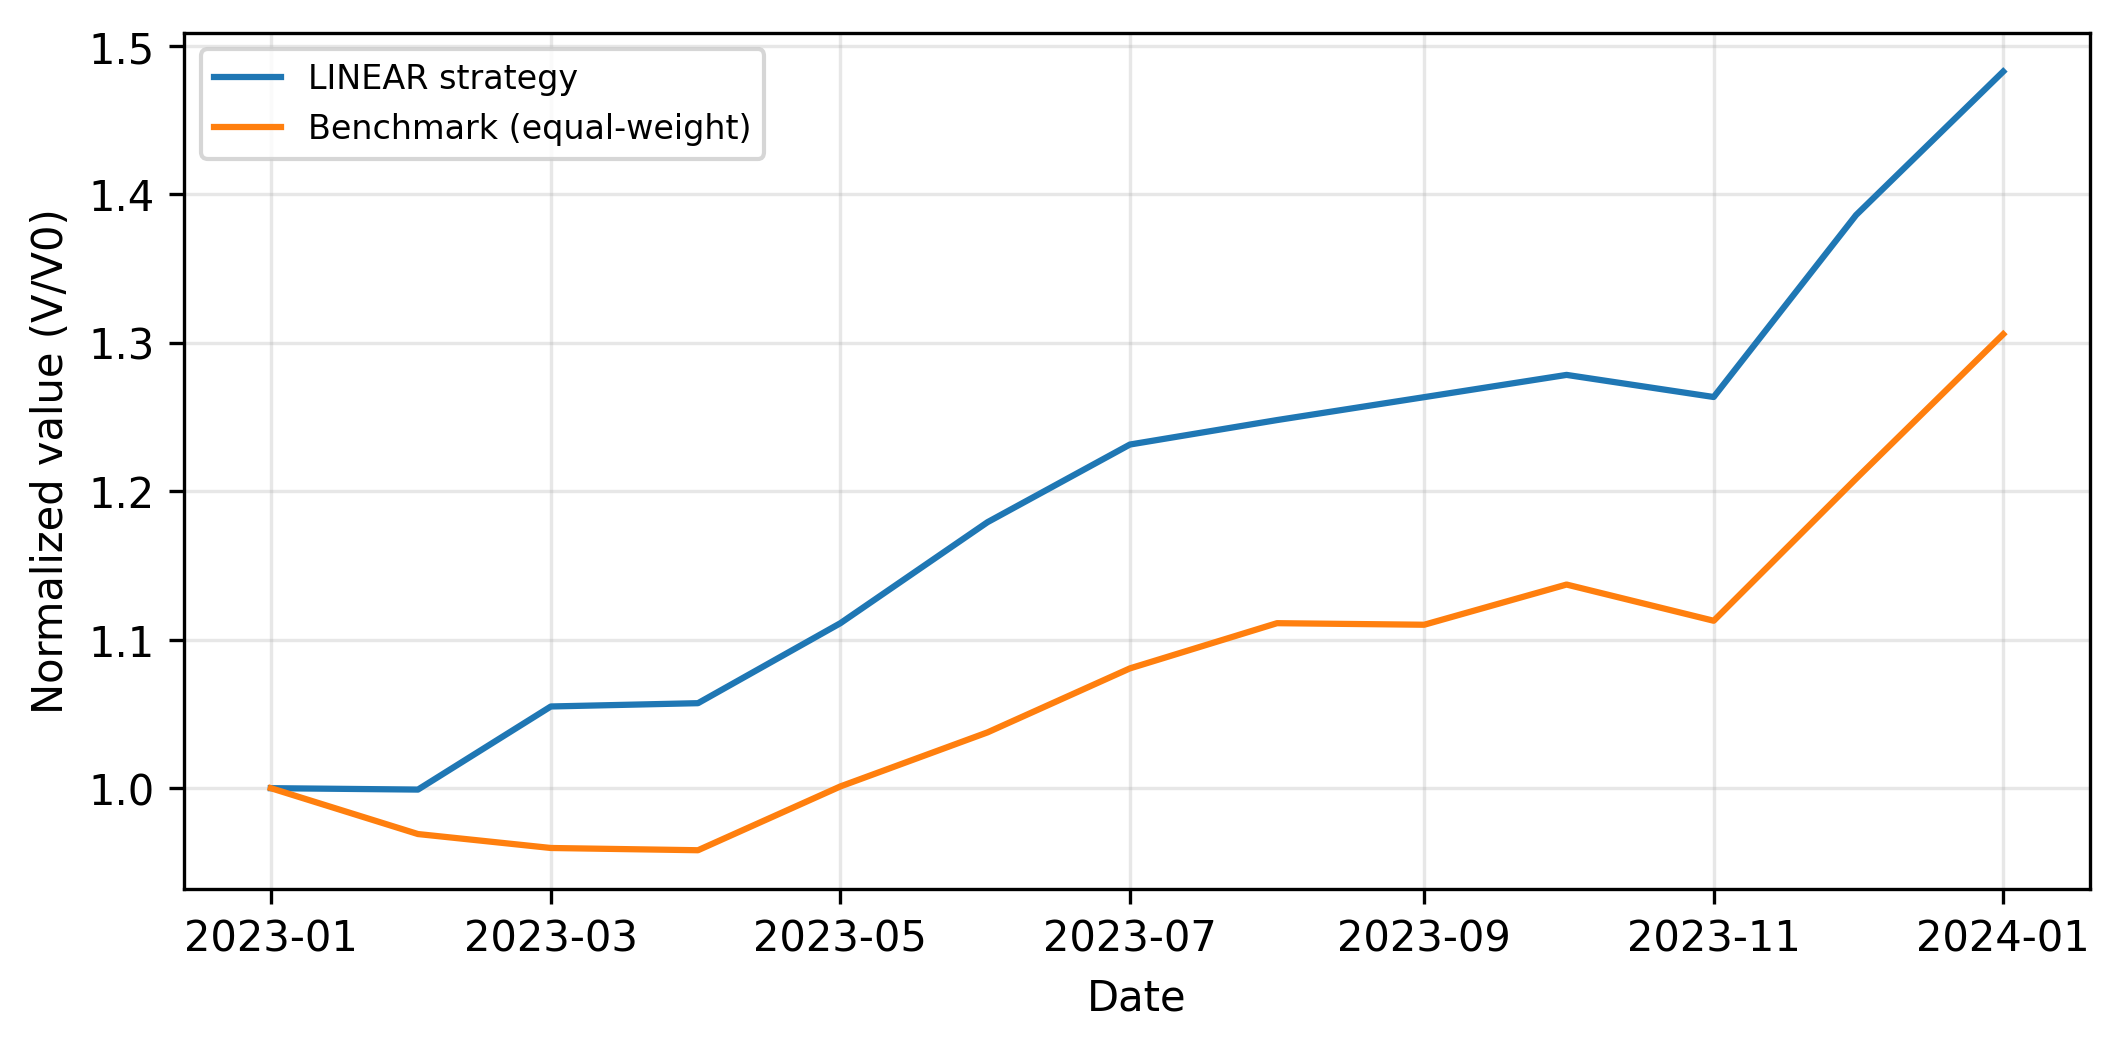
\includegraphics[width=\columnwidth]{figures/equity_curve_2023_2024_linear.png}
\caption{Normalized equity curve for the implemented LINEAR strategy vs. the equal-weight benchmark (monthly rebalancing, 2023-01-01 to 2024-01-01).}
\label{fig:equitycurve}
\end{figure}

\begin{figure}[!t]
\centering
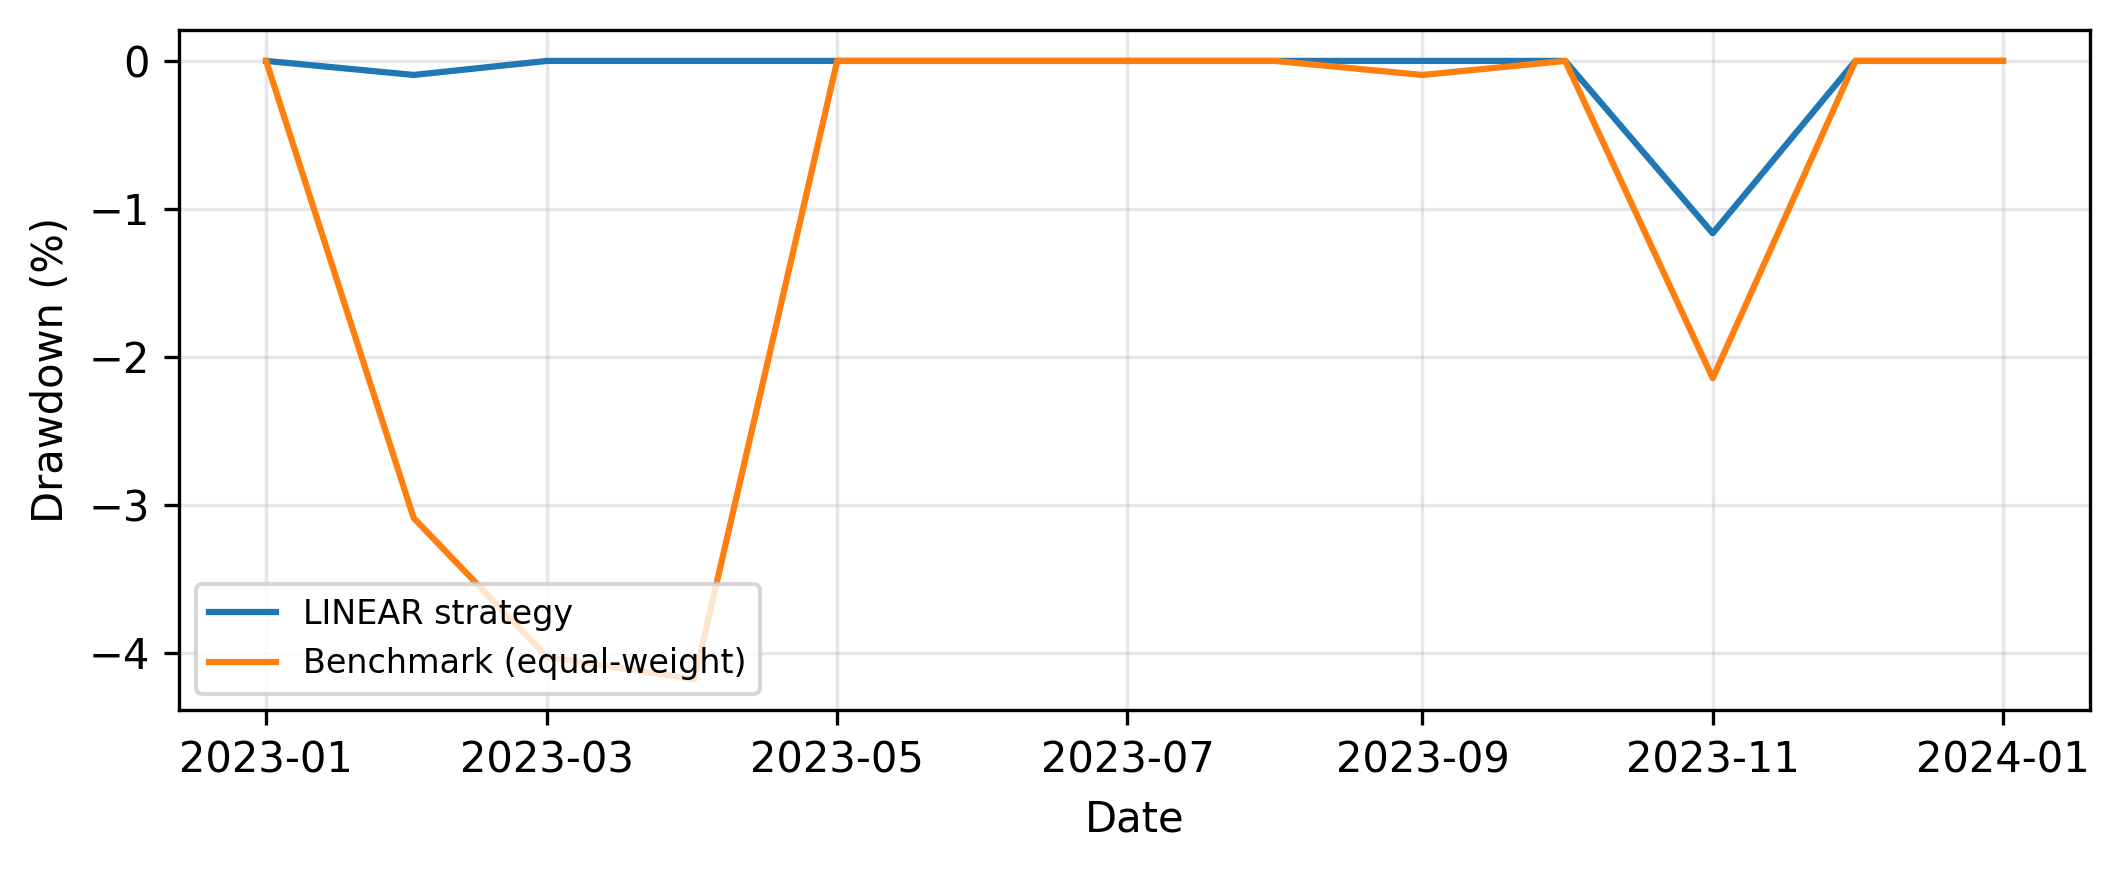
\includegraphics[width=\columnwidth]{figures/drawdown_2023_2024_linear.png}
\caption{Drawdown comparison for the implemented LINEAR strategy vs. the equal-weight benchmark over the same walk-forward run.}
\label{fig:drawdown}
\end{figure}

\begin{table}[!t]
\centering
\caption{Walk-forward backtest summary (monthly rebalancing, 2023-01-01 to 2024-01-01).}
\label{tab:backtest}
\small
\setlength{\tabcolsep}{4pt}
\renewcommand{\arraystretch}{1.15}
\begin{tabularx}{\columnwidth}{|X|c|c|c|}
\hline
\textbf{Portfolio} & \textbf{CAGR} & \textbf{Sharpe} & \textbf{Max DD} \\
\hline
LINEAR Strategy & 48.31\% & 3.04 & -1.17\% \\
Benchmark (equal-weight) & 30.60\% & 1.75 & -4.18\% \\
\hline
\end{tabularx}
\end{table}

\subsection{Discussion}
The reported metrics highlight known challenges in financial prediction: noisy labels, regime shifts, and weak signal-to-noise ratios. Negative test $R^2$ for the regression baseline indicates that naive baselines can outperform poorly specified targets on some splits. QuantFin mitigates common failure modes by making preprocessing and evaluation explicit and repeatable, exposing multiple model families for comparison, and emphasizing risk-adjusted backtest metrics rather than a single accuracy value.

\subsection{Limitations observed in the current codebase}
QuantFin is intended as an end-to-end educational and prototyping platform, and the repository reflects this stage. For example, the backend validation report included in the repository indicates some integration checks are not passing, and production readiness is explicitly marked as false. In addition, backtests currently omit explicit transaction cost and slippage modeling, which can materially affect realized performance.

\subsection{Threats to validity}
While QuantFin enforces time-ordered cutoffs in walk-forward evaluation, several threats remain that can inflate or destabilize results if not addressed: (i) the absence of transaction costs, slippage, and liquidity constraints in the current backtest; (ii) simplified covariance assumptions in some optimization baselines (e.g., constant-correlation covariance in the prediction service); and (iii) model-selection and hyperparameter choices that may implicitly tune to a particular market regime. These limitations are documented here to keep interpretation aligned with the repository's current implementation.

\FloatBarrier

\section{Conclusion}\label{sec:con}
This paper presented QuantFin, a machine learning--based decision support system for investments that integrates data preprocessing, feature engineering, multi-model prediction, portfolio construction, and walk-forward backtesting for Nifty~50 equities available in the repository dataset. The system provides practical APIs and an interactive dashboard, enabling users to compare models, rebalance portfolios, and validate performance against a benchmark.

Current results demonstrate that the end-to-end pipeline is functional and produces measurable baselines. The platform's outputs should be interpreted as decision support rather than a guarantee of profit: predictive performance remains limited by market non-stationarity, and the backtest currently omits transaction costs and slippage. Future work includes improving label design, adding transaction-cost modeling, and integrating the repository's auxiliary news dataset into the feature pipeline only once it is wired into the active prediction/portfolio flow.

\bibliographystyle{IEEEtran}
%\fontsize{10}{10}\selectfont
%\addcontentsline{toc}{section}{\textbf{REFERENCES}}
%\renewcommand{\bibname}{REFERENCES}
\bibliography{review}
%\end{spacing}
\end{document}
